% Version 3 December 2023
% See section 11 of the User Manual for version history
%
%%%%%%%%%%%%%%%%%%%%%%%%%%%%%%%%%%%%%%%%%%%%%%%%%%%%%%%%%%%%%%%%%%%%%%
%%                                                                 %%
%% Please do not use \input{...} to include other tex files.       %%
%% Submit your LaTeX manuscript as one .tex document.              %%
%%                                                                 %%
%% All additional figures and files should be attached             %%
%% separately and not embedded in the \TeX\ document itself.       %%
%%                                                                 %%
%%%%%%%%%%%%%%%%%%%%%%%%%%%%%%%%%%%%%%%%%%%%%%%%%%%%%%%%%%%%%%%%%%%%%

% \documentclass[referee,sn-basic]{sn-jnl}% referee option is meant for double line spacing

%%=======================================================%%
%% to print line numbers in the margin use lineno option %%
%%=======================================================%%

% \documentclass[lineno,sn-basic]{sn-jnl}% Basic Springer Nature Reference Style/Chemistry Reference Style

%%======================================================%%
%% to compile with pdflatex/xelatex use pdflatex option %%
%%======================================================%%

%%\documentclass[pdflatex,sn-basic]{sn-jnl}% Basic Springer Nature Reference Style/Chemistry Reference Style

%%Note: the following reference styles support Namedate and Numbered referencing. By default the style follows the most common style. To switch between the options you can add or remove “Numbered” in the optional parenthesis.\\

%%The option is available for: sn-basic.bst, sn-vancouver.bst, sn-chicago.bst%

\documentclass[pdflatex,sn-nature, lineno]{sn-jnl}% Style for submissions to Nature Portfolio journals
% \documentclass[pdflatex,sn-basic]{sn-jnl}% Basic Springer Nature Reference Style/Chemistry Reference Style
% \documentclass[pdflatex, sn-mathphys-num, lineno]{sn-jnl}% Math and Physical Sciences Numbered Reference Style
%%\documentclass[pdflatex,sn-mathphys-ay]{sn-jnl}% Math and Physical Sciences Author Year Reference Style
%%\documentclass[pdflatex,sn-aps]{sn-jnl}% American Physical Society (APS) Reference Style
%%\documentclass[pdflatex,sn-vancouver,Numbered]{sn-jnl}% Vancouver Reference Style
%%\documentclass[pdflatex,sn-apa]{sn-jnl}% APA Reference Style
%%\documentclass[pdflatex,sn-chicago]{sn-jnl}% Chicago-based Humanities Reference Style

%%%% Standard Packages
%% additional latex packages if required can be included here>
\usepackage{graphicx}%
\usepackage{multirow}%
\usepackage{amsmath,amssymb,amsfonts}%
\usepackage{amsthm}%
\usepackage{mathrsfs}%
\usepackage[title]{appendix}%
\usepackage{xcolor}%
\usepackage{textcomp}%
\usepackage{manyfoot}%
\usepackage{booktabs}%
\usepackage{algorithm}%
\usepackage{algorithmicx}%
\usepackage{algpseudocode}%
\usepackage{listings}%

\usepackage{xspace}
\usepackage{standalone}

%% my package start

% for collabration and will remove before submit
\newcommand{\yy}[1]{\textcolor{cyan}{\textbf{[Yangyang: #1]}}}
\newcommand{\rd}[1]{\textcolor{green}{\textbf{[Dr.Yang: #1]}}}
\newcommand{\ty}[1]{\textcolor{orange}{\textbf{[Tingyou: #1]}}}
\newcommand{\qx}[1]{\textcolor{purple}{\textbf{[Qingxiang: #1]}}}

% for collabration and will remove before submit

\usepackage[detect-all=true]{siunitx}
\sisetup{
    scientific-notation=false,
    round-mode = places,
    round-precision = 0
}

\usepackage[acronym, automake, style=index, shortcuts]{glossaries-extra}
\setabbreviationstyle[acronym]{long-short}
% define glossaries
\makeglossaries

\newacronym{blat}{BLAT}{BLAST-like alignment tool}
\newacronym{llm}{LLM}{Large Language Model}
\newacronym{hmm}{HMM}{Hidden Markov Model}
\newacronym{gpu}{GPU}{Graphics Processing Unit}
\newacronym{hpc}{HPC}{High Performance Computing}
\newacronym{bert}{BERT}{Bidirectional Encoder Representations from Transformers}
\newacronym{gpt}{GPT}{Generative Pre-trained Transformer}

\newacronym{ide}{IDE}{Integrated Development Environment}
\newacronym{cd}{CD}{Continuous Development}
\newacronym{ucsc}{UCSC}{UCSC Genome Browser}
\newacronym{glm}{GLM}{Genomic Language Model}
\newacronym{lcglm}{LCGLM}{long-context genomic language model}
\newacronym{snp}{SNP}{Single Nucleotide Polymorphism}
\newacronym{fm}{FM}{Foundational Model}
\newacronym{nlp}{NLP}{Natural Language Processing}

\newacronym{mlp}{MLP}{multilayer perceptron}
\newacronym{drs}{dRNA-seq}{direct RNA sequencing}
\newacronym{ont}{ONT}{Oxford Nanopore Technologies}
\newacronym{pb}{PacBio}{Pacific Biosciences}

\newacronym{go}{GO}{Gene Ontology}
\newacronym{r2c2}{R2C2}{Rolling Circle Amplification to Concatemeric Consensus}
\newacronym{pcr}{PCR}{Polymerase Chain Reaction}

\newacronym{fsm}{FMS}{Full splice match}
\newacronym{ism}{ISM}{Incomplete splice match}
\newacronym{nic}{NIC}{Novel in catalog}
\newacronym{nnc}{NNC}{Novel not in catalog}

\newacronym{tp}{TP}{True Positive}
\newacronym{fp}{FP}{False Positive}
\newacronym{fn}{FN}{False Negative}

\newacronym{mrna}{mRNA}{messenger RNA}
\newacronym{rta}{RTA}{reverse transcriptase adapter}

\newcommand{\figref}[2]{Fig.~\hyperref[#1]{\ref*{#1}#2}}
\newcommand{\edfigref}[2]{Extended Data Fig.~\hyperref[#1]{\ref*{#1}#2}}
\newcommand{\edfigrefrg}[3]{Extended Data Fig.~\hyperref[#1]{\ref*{#1}#2-\ref*{#1}#3}}

\graphicspath{{../figures}}
%% my package end


%%%%%=============================================================================%%%%
%%%%  Remarks: This template is provided to aid authors with the preparation
%%%%  of original research articles intended for submission to journals published
%%%%  by Springer Nature. The guidance has been prepared in partnership with
%%%%  production teams to conform to Springer Nature technical requirements.
%%%%  Editorial and presentation requirements differ among journal portfolios and
%%%%  research disciplines. You may find sections in this template are irrelevant
%%%%  to your work and are empowered to omit any such section if allowed by the
%%%%  journal you intend to submit to. The submission guidelines and policies
%%%%  of the journal take precedence. A detailed User Manual is available in the
%%%%  template package for technical guidance.
%%%%%=============================================================================%%%%

%% as per the requirement new theorem styles can be included as shown below
\theoremstyle{thmstyleone}%
\newtheorem{theorem}{Theorem}%  meant for continuous numbers
%%\newtheorem{theorem}{Theorem}[section]% meant for sectionwise numbers
%% optional argument [theorem] produces theorem numbering sequence instead of independent numbers for Proposition
\newtheorem{proposition}[theorem]{Proposition}%
%%\newtheorem{proposition}{Proposition}% to get separate numbers for theorem and proposition etc.

\theoremstyle{thmstyletwo}%
\newtheorem{example}{Example}%
\newtheorem{remark}{Remark}%

\theoremstyle{thmstylethree}%
\newtheorem{definition}{Definition}%

\raggedbottom
\unnumbered% uncomment this for unnumbered level heads

\begin{document}

\title[Article Title]{A Genomic Language Model for Chimera Artifact Detection in Nanopore Direct RNA Sequencing}

%%=============================================================%%
%% GivenName	-> \fnm{Joergen W.}
%% Particle	-> \spfx{van der} -> surname prefix
%% FamilyName	-> \sur{Ploeg}
%% Suffix	-> \sfx{IV}
%% \author*[1,2]{\fnm{Joergen W.} \spfx{van der} \sur{Ploeg}
%%  \sfx{IV}}\email{iauthor@gmail.com}
%%=============================================================%%

\author[1]{\fnm{Yangyang} \sur{Li}}\email{yangyang.li@northwestern.edu}
\equalcont{These authors contributed equally to this work.}

% \author*[1,2]{\fnm{First} \sur{Author}}\email{iauthor@gmail.com}
\author[1]{\fnm{Ting-You} \sur{Wang}}\email{tywang@northwestern.edu}
\equalcont{These authors contributed equally to this work.}

\author[1]{\fnm{Qingxiang} \sur{Guo}}\email{qingxiang.guo@northwestern.edu}

\author[1]{\fnm{Yanan} \sur{Ren}}\email{ynren1020@gmail.com}
\author[1]{\fnm{Xiaotong} \sur{Lu}}\email{xiaotong.lu@northwestern.edu}

\author[1,2]{\fnm{Qi} \sur{Cao}}\email{qi.cao@northwestern.edu}
\author*[1,2]{\fnm{Rendong} \sur{Yang}}\email{rendong.yang@northwestern.edu}

\affil[1]{\orgdiv{Department of Urology}, \orgname{Northwestern University Feinberg School of Medicine}, \orgaddress{\street{303 E Superior St}, \city{Chicago}, \postcode{60611}, \state{IL}, \country{USA}}}
\affil[2]{\orgdiv{Robert H. Lurie Comprehensive Cancer Center}, \orgname{Northwestern University Feinberg School of Medicine}, \orgaddress{\street{675 N St Clair St}, \city{Chicago}, \postcode{60611}, \state{IL}, \country{USA}}}

% \author[1,2]{\fnm{Third} \sur{Author}}\email{iiiauthor@gmail.com}
% \equalcont{These authors contributed equally to this work.}

% \affil*[1]{\orgdiv{Department}, \orgname{Organization}, \orgaddress{\street{Street}, \city{City}, \postcode{100190}, \state{State}, \country{Country}}}
% \affil[2]{\orgdiv{Department}, \orgname{Organization}, \orgaddress{\street{Street}, \city{City}, \postcode{10587}, \state{State}, \country{Country}}}
% \affil[3]{\orgdiv{Department}, \orgname{Organization}, \orgaddress{\street{Street}, \city{City}, \postcode{610101}, \state{State}, \country{Country}}}

%%==================================%%
%% Sample for unstructured abstract %%
%%==================================%%

\abstract{
	Nanopore \gls{drs} has revolutionized transcriptomics but is challenged by artificial chimeric reads that compromise data integrity.
	We present DeepChopper, a novel large language model tailored for biological sequences, which accurately identifies and removes artificial sequences in nanopore \gls{drs} data without relying on alignment information.
	DeepChopper includes long-range dependency modeling with quality-aware processing and achieves both broad context understanding and single-nucleotide resolution.
        Across multiple cell lines and sequencing platforms, DeepChopper reduced chimeric reads by 62-84\% and improved supporting rates from 8-19\% to 43-55\% compared to existing methods.
	In particular, in gene fusion detection, DeepChopper reduced false positives by 89\% while increasing the proportion of supported fusions from 2\% to 17\%.
	By improving data quality, DeepChopper significantly improves the reliability of downstream analyses, particularly in cancer genomics and transcriptomics.
	This work demonstrates the powerful potential of large language models in analyzing complex biological data, paving the way for advancements in genomics and biotechnology.}
\maketitle

\section{Main}

% Outline
% 1. Sequencing history
% 2. Genomics LLM history
% 3. Challenges of LLM / efficiency of transformer and improvements
% 3.1 long range
% 3.2 single nucleotide resolution
% 4. Cons of drs
% 5. Our method
% 6. Results
% 7. Conclusion

Long-read RNA sequencing technologies are revolutionizing transcriptomic research by providing unparalleled resolution for detecting complex splicing and gene fusion events often missed by conventional short-read RNA-seq methods.
Among these technologies, \gls{ont} \gls{drs} stands out by sequencing full-length RNA molecules directly, preserving native RNA modifications and allowing a more accurate and comprehensive analysis of RNA biology.
This approach bypasses the inherent limitations of cDNA-based sequencing methods, such as artifacts arising from reverse transcription, template switching, and \gls{pcr} amplification~\cite{garalde2018highly, jain2022advances}.

Despite these advantages, a critical question remains: Does \gls{ont} \gls{drs} introduce technical artifacts?
A previous study has suggested that \gls{drs} might generate chimera artifacts, leading to multi-mapped reads~\cite{smith2020molecular}.
These artifacts may result from ligation during library preparation or chimeric reads produced by software missing the open pore signal, potentially confounding downstream analyses such as transcriptome assembly, quantification, and detection of alternative splicing and gene fusion events.
Detecting these chimera artifacts is challenging because long-read aligners often produce chimeric alignments from such artifacts that are indistinguishable from those derived from true gene fusion events.
Importantly, chimeric read artifacts frequently contain internal adapter sequences~\cite{smith2020molecular}, which could theoretically serve as a distinguishing feature to differentiate them from true gene fusion-derived reads.
However, \gls{ont} \gls{drs} basecallers, trained in RNA, struggle to properly call these DNA-based adapter sequences under an RNA model~\cite{liu2024sequencing}.
As a result, current adapter detection tools cannot exploit this feature to eliminate chimeric read artifacts, leaving the issue unresolved.

To address these challenges, we developed DeepChopper, a \gls{glm} specifically designed for long-read sequence analysis.
Inspired by recent advances in \gls{llm} that can decipher complex patterns in genetic sequences~\cite{benegas2024genomic}, DeepChopper excels at processing long genomic contexts with single-nucleotide resolution, a crucial capability for identifying \gls{ont} adapter sequences directly from base-called long reads and thus facilitating the detection and removal of chimeric read artifacts in \gls{drs} data.
Specifically, DeepChopper processes individual FASTQ records to identify and handle adapter sequences: When internal adapters are detected, the model splits the read into two or more records, while $3'$ end adapters are trimmed to produce a clean sequence (\figref{fig:f1}{a}).
This method ensures the preservation of genuine biological sequences while effectively eliminating chimera artifacts. 

To accomplish this, DeepChopper integrates the \gls{lcglm} HyenaDNA~\cite{nguyen2024hyenadna}, optimized for efficient long-range dependency modeling, with a residual block and a \gls{mlp} for fine-grained sequence analysis.
This hybrid architecture enables both broad context understanding and precise single-nucleotide resolution~\cite{poli2023hyena, he2016deep} (\figref{fig:f1}{a}).
Additionally, DeepChopper incorporates base quality score information to improve prediction and employs an adaptive tokenization strategy that preserves single-nucleotide resolution while capturing higher-order sequence patterns (See \hyperref[sec:methods]{Methods} for details).
DeepChopper offers several advantages over existing genomic language models.
Unlike DNABERT2~\cite{zhou2023dnabert2}, which is limited to a context length of 512 base pairs, DeepChopper processes up to 32 kilobase pairs, a sufficiently long context to capture most mRNAs.
Additionally, unlike Nucleotide Transformer~\cite{dalla2023nucleotide}, which lacks single-base resolution, DeepChopper can accurately identify non-human reference sequences, such as \gls{ont} adapters, with base-pair precision. 
Moreover, its efficient architecture—using only 7 million parameters—makes DeepChopper computationally practical for large-scale \gls{drs} analysis, in contrast to resource-intensive models like Evo~\cite{nguyen2024sequence}, which rely on billions of parameters and may not be feasible in environments with limited computational resources.
This combination of long context processing, high-resolution accuracy, and computational efficiency makes DeepChopper particularly well-suited for analyzing massive long-read sequences.

% Result
\begin{figure}[!h]
	\includegraphics[height=0.78\columnwidth]{finals/figure1}
	\caption{{\bf  Detection of chimeric read artifacts in \gls{drs} data using DeepChopper and validation with orthogonal sequencing platforms} (a) Overview of the architecture of the DeepChopper model. Created with BioRender.com (b) Length distribution of predicted adapters by DeepChopper in VCaP \gls{drs} data. (c) Distribution of relative adapter position along read length in VCaP \gls{drs} data. Grey rectangle represents a long read from $5'$ to $3'$. Relative position is calculated as the ratio of the length before DeepChopper predicted adapter start position to the total read length. (d) Distribution of segments per read after trimming: 1 segment indicates $3'$ end adapter trimmed, while 2 or more indicate internal adapters trimmed. (e) Chimeric alignments (in thousands) for VCaP \gls{drs} reads processed by Dorado with and without adapter trimming, and DeepChopper. DeepChopper greatly reduces chimeric alignments not supported by direct cDNA sequencing. (f) Distribution of base qualities from identified internal adapters by DeepChopper. Background colors indicate quality levels: green (high), yellow (medium), and red (low). (g) \gls{blat} identity distribution of the internal adapter sequences mapping against human reference genome. (h) The number of chimeric alignments (in thousands) for A549, HCT116, HepG2, K562, and MCF7 cell lines processed by Dorado with adapter trimming and DeepChopper. DeepChopper consistently reduces chimeric alignments not supported by cDNA sequencing across all cell lines. (i) Chimeric alignments from \gls{drs} of the WTC11 cell line, evaluated for support using additional \gls{ont} and \gls{pb} sequencing data with different protocols. DeepChopper reduces unsupported chimeric alignments across all methods compared to Dorado with adapter trimming.}\label{fig:f1}
\end{figure}

To train DeepChopper for identifying adapter sequences within \gls{drs} long reads, we utilized data from six human cell lines: HEK293T, A549, HCT116, HepG2, K562 and MCF-7 provided by the Singapore Nanopore Expression Project (SG-NEx)~\cite{chen2021systematic}.
We curated a training set of 540,000 long reads initially deemed free of adapters and inserted putative adapter sequences, derived from the raw \gls{drs} data, into these reads to create instances containing internal and $3'$ end adapters (See \hyperref[sec:methods]{Methods} for details).
An independent test set comprising 60,000 long reads was held out for performance evaluation.
DeepChopper achieved recall, precision, and F1 scores above 0.99 (\edfigref{fig:sf1}{a}), demonstrating its high accuracy in detecting adapter sequences.
To further assess DeepChopper’s ability to detect chimera artifacts in real data, we generated an additional \gls{drs} dataset using the prostate cancer VCaP cell line, which was not included in the training data.
This independent dataset provides a robust framework for evaluating chimera artifacts in genuine \gls{drs} samples, ensuring that DeepChopper's performance generalizes beyond the training data. 

We conducted \gls{drs} of VCaP cells using \gls{ont}'s SQK-RNA002 chemistry, consistent with that used in the SG-NEx project.
Using a MinION sequencer with four R9.4 flow cells, we generated a total of 9,177,639 long reads in FASTQ format, with base-calling performed by \gls{ont}'s Dorado software~\cite{dorado2023}.
DeepChopper was then applied for adapter trimming and correction of chimeric read artifacts.
Notably, DeepChopper increased the yield of long-read sequences by 3\%, resulting in a final output of 9,357,913 long reads.
DeepChopper identified 8,218,172 adapter sequences within 7,990,102 long reads, accounting for 87\% of the raw reads. 
Most of these adapter sequences were approximately 70 bp in length (\figref{fig:f1}{b}), aligning with the expected length of the RMX adapter used in \gls{ont} SQK-RNA002 \gls{drs} kit, as specified in the kit's technical documentation~\cite{nano2017tech}.

We then analyzed the positions of DeepChopper identified adapter sequences within each long read.
Among these, 212,478 reads contained internal adapters, while 7,777,624 reads had adapters at their $3'$ ends (\figref{fig:f1}{c}).
This reveals that chimeric read artifacts, evidenced by internal adapters, are present in VCaP \gls{drs} data and may reflect a common problem inherent to \gls{drs} long reads.
Further examination of adapter-trimmed reads showed that chimera artifacts could arise from the joining of multiple long reads, with the most prevalent type involving two reads connected by an internal adapter to form a single chimeric read (\figref{fig:f1}{d}).

To validate the chimeric read artifacts identified by DeepChopper in the VCaP \gls{drs} data, we analyzed the chimeric alignments generated by minimap2\cite{li2018minimap2}, as chimeric reads typically produce such alignments.
To distinguish genuine chimeric reads from artifacts, we generated Nanopore direct cDNA sequencing data for VCaP cells and considered chimeric reads with alignments fully supported by cDNA sequencing as bona fide (See \hyperref[sec:methods]{Methods} for details).
Additionally, we assessed whether the adapter trimming function of \gls{ont}'s Dorado basecaller could mitigate chimeric read artifacts.
While Dorado's adapter trimming had no effect on reducing chimeric alignments, DeepChopper achieved a 91\% reduction and increased the proportion of cDNA-supported chimeric alignments from 5\% to 47\% (\figref{fig:f1}{e}).
To further confirm the nature of the identified chimeric read artifacts, we examined the base quality scores of the internal adapter sequences identified by DeepChopper and aligned them with the human reference genome using \gls{blat}~\cite{kent2002blat}, a tool known for its high alignment accuracy.
Our analysis revealed that the adapter sequences from the chimeric read artifacts exhibited low base quality scores (\figref{fig:f1}{f}) and poor alignment identity with the human reference genome (\figref{fig:f1}{g}), confirming their artifactual nature and non-human origin.

To comprehensively assess DeepChopper’s performance in reducing chimera artifacts in \gls{drs}, we examined cDNA-supported chimeric alignments in the SG-NEx samples. 
DeepChopper significantly reduced chimeric alignments by 62\% to 84\%, while preserving cDNA-supported chimeric alignments without noticeable reduction (\figref{fig:f1}{h}), indicating the prevalence of chimeric read artifacts in \gls{drs}. 

To further validate DeepChopper's accuracy, we applied it to process \gls{drs} data from the human WTC11 induced pluripotent stem cell line, generated by the LRGASP project~\cite{pardo2024systematic}.
Additionally, the LRGASP project generated cDNA-based long-read sequencing data from this cell line using distinct protocols (\gls{pcr}-cDNA, CapTrap, \gls{r2c2}) on both \gls{ont} and \gls{pb} platforms, providing a valuable resource for benchmarking DeepChopper's performance.
We observed that DeepChopper consistently eliminated only the chimeric alignments in the \gls{drs} data that were not supported by any cDNA-based sequencing method (\figref{fig:f1}{i}), demonstrating its precise ability to distinguish genuine chimeric reads from artifacts.

Recently, \gls{ont} released a new SQK-RNA004 chemistry for \gls{drs}, but it remains unclear whether chimera artifacts persist with this update. 
To investigate, we generated \gls{drs} data using the latest SQK-RNA004 kit for the VCaP cell line and performed zero-shot predictions of chimera artifacts using DeepChopper, despite the adapter sequence pattern of RNA004 not being included in its training.
DeepChopper reduced chimeric alignments by 21\% compared to Dorado's base-called and adapter-trimmed long reads, increasing the proportion of cDNA-supported chimeric alignments from about 25\% to 30\% (\edfigref{fig:sf1}{b}).
Furthermore, the internal adapter sequences identified by DeepChopper within these RNA004 chimeric read artifacts exhibited low base quality scores (with a mean of 7.8) and low \gls{blat} identity (mean of 0.38) (\edfigref{fig:sf1}{c}).
These findings strongly suggest that chimera artifacts persist in the latest RNA004 \gls{drs} kit.

\begin{figure}[H]
	\includegraphics[height=1\columnwidth]{finals/figure2}
	\caption{{\bf Characterization of \gls{drs} chimera artifacts and their impact on downstream analysis in VCaP cells} (a) The upper bar plot shows the number of chimeric connections per kilobase across chromosomes, highlighting higher chimeric activity in Chr 19 and Chr M. The lower heatmap visualizes interchromosomal connections, with intensity indicating the count of connections between different chromosomes. (b) The bar plot shows the number of transcripts (in thousands) across different isoform classification categories. DeepChopper-processed reads result in a higher number of transcripts compared to Dorado-trimmed reads. The inset details the isoform classification scheme. (c) Detected gene fusions from Dorado adapter-trimmed reads and DeepChopper-processed reads. Gene fusions identified from short-read RNA-seq were used to validate fusion events detected from \gls{drs}. (d) \gls{go} enrichment analysis of chimera artifact-affected genes, with color indicating gene count per term. (e) Analysis of a chimeric read artifact detected as an RPS29-COX8A fusion. The schematic shows the fusion between RPS29 (Chr 14) and COX8A (Chr 11). The green plot indicates quality scores along the read, and the blue plot shows raw signal intensity (in pA). The chopped region identified by DeepChopper corresponds to a low-quality segment with low current intensity, polyA, and short open pore signals, suggesting the presence of an \gls{ont} adapter.}\label{fig:f2}
\end{figure}

To investigate potential factors contributing to the formation of chimera artifacts, we examined the expression levels and sizes of the genes involved in these artifacts, we found that genes affected by chimera artifacts exhibited significantly higher expression levels compared to all expressed genes (\(\textrm{p-value} < 2.2 \times 10^{-16}\)) (\edfigref{fig:sf2}{a}), while following a similar size distribution pattern (\edfigref{fig:sf2}{b}).
We then analyzed the genomic patterns of improper connections generated by chimera artifacts across chromosomes in VCaP \gls{drs} data.
These artifacts showed varying frequencies across chromosomes, with the mitochondrial chromosome (Chr M) exhibiting an especially high rate of connections per base pair, indicating it may be a hotspot for chimera artifact formation (\figref{fig:f2}{a}).
A similar pattern of improper inter-chromosomal connections was also observed in VCaP RNA004 \gls{drs} data (\edfigref{fig:sf2}{c}), suggesting that chimera artifacts may be an inherent issue of \gls{drs} technology, rather than being fully resolved by improvements in sequencing chemistry.

To evaluate the influence of chimera artifacts on downstream analyses, we investigated the impact of DeepChopper-mediated correction on transcript annotation. IsoQuant~\cite{prjibelski2023accurate} was employed to detect and annotate transcripts from VCaP dRNA-seq data, focusing on chimeric read artifacts identified by DeepChopper. By comparing transcript identification with and without DeepChopper correction, we observed a substantial increase in the number of identified transcripts (\figref{fig:f2}{b}). Similarly, an increase in transcript detection was observed in VCaP dRNA-seq data generated using the latest RNA004 kit (\edfigref{fig:sf2}{d}). The increase in detected transcripts was most prominent in the full-length transcripts (\gls{fsm} category), with additional improvements noted across the alternatively spliced transcript categories (\gls{ism}, \gls{nic}, and \gls{nnc}). These findings underscore the effectiveness of DeepChopper in mitigating the detrimental effects of chimera artifacts on transcript annotation.

Finally, we evaluated whether DeepChopper could improve gene fusion detection by chimera artifact correction.
Gene fusion calls detected by FusionSeeker~\cite{chen2023gene} from DeepChopper-processed \gls{drs} reads showed a 89\% reduction compared to those from adapter-trimmed dRNA-seq reads processed by Dorado.
To further assess this reduction, we applied Arriba~\cite{uhrig2021accurate} to detect gene fusions using short-read RNA-seq of VCaP cells and found that none of the gene fusion calls reduced by DeepChopper were supported by those detected in RNA-seq data (\figref{fig:f2}{c}).
This demonstrates that DeepChopper effectively reduces false positive gene fusion calls caused by chimera artifacts in \gls{drs}— an essential improvement for accurately identifying gene fusion drivers in cancer transcriptomes.

Upon closer examination of the chimera artifact-derived gene fusion calls, we found a notable enrichment of ribosomal protein genes (\edfigref{fig:sf3}{a}).
GO enrichment analysis in VCaP (\figref{fig:f2}{d}) and SG-NEx cell lines (\edfigref{fig:sf3}{b}) confirmed that housekeeping ribosomal protein genes are frequently involved in these artifacts.
Additionally, we manually inspected a chimeric read identified as an RPS29-COX8A fusion involving the 40S ribosomal protein S29 in the VCaP dRNA-seq data.
The DeepChopper-chopped region aligned with raw current signals showing low intensity, indicative of \gls{ont} adapters (\figref{fig:f2}{e}).
The presence of polyA and open pore signals at the boundary of this region further suggested that this chimeric read resulted from improperly joined mRNA transcripts rather than a genuine gene fusion event.

In conclusion, DeepChopper demonstrates a significant potential for leveraging \gls{llm} to analyze long-read sequences, particularly by addressing the previously overlooked issue of chimera artifacts in Nanopore \gls{drs}.
DeepChopper significantly enhances the quality of the \gls{drs} data by identifying and removing \gls{ont} adapters directly from the base-called long-read sequences, thereby boosting the precision of subsequent transcript and gene fusion analyses.
This advancement not only optimizes current nanopore \gls{drs} analysis but also highlights the broader applicability of language models to address the complex biological challenges posed by emerging long-read technologies.

\section{Methods}\label{sec:methods}

\subsection{Cell culture}

VCaP cell line was obtained from the American Type Culture Collection (ATCC) and cultured under sterile conditions to maintain optimal growth and viability.
The cells were grown in Dulbecco's Modified Eagle Medium (DMEM, high glucose; Gibco, Cat\# 11-965-092) supplemented with 10\% fetal bovine serum (FBS Opti-Gold, Performance Enhanced, US Origin; Gendepot, Cat\# F0900-050) to provide essential growth factors.
In addition, the culture medium was enriched with \SI{5}{\ml} of 100 mM Sodium Pyruvate (Gendepot, Cat\# CA017-010) to support cellular metabolism and \SI{5}{\ml} of Antibiotics-Antimycotics (\( 100\times \)) (Gendepot, Cat\# CA002-010) to prevent microbial contamination.
Cells were cultured in \SI{100}{\mm} cell culture treated dishes (Thermo Fisher Scientific, Cat\# 12-556-002) and incubated at \SI{37}{\degreeCelsius} in a humidified atmosphere containing 5\% CO2, with media changes performed every 72 hours to ensure nutrient availability and waste removal.
Cell confluency was regularly monitored and subculturing was performed before reaching 80\% confluency to maintain healthy growth conditions and prevent over-confluence stress.

\subsection{RNA extraction and quantification}

Total RNA was extracted using the RNeasy Mini Kit (Qiagen, Cat\# 74104) according to the protocol of the manufacturer.
The quality and concentration of RNA were assessed using an Agilent 2100 Bioanalyzer.
Poly(A)+ RNA was then enriched from total RNA using the Dynabeads\textsuperscript{tm} mRNA Purification Kit (Invitrogen, Cat\# 65001), which utilizes oligo (dT) beads for selective mRNA binding.
The mRNA was quantified using a Qubit 4 fluorometer and a Qubit RNA HS Assay Kit (Thermo Fisher Scientific, Cat\# Q32852).
The mRNA preparations were either immediately used to prepare a sequencing library or frozen and stored at \SI{-80}{\degreeCelsius} until further use.

\subsection{Nanopore sequencing}

We performed Direct-RNA nanopore sequencing of the enriched mRNA using two different sets: the RNA002 kits with R9.4.1 flow cells and the RNA004 kits with R10.4.1 flow cells.
The decision to incorporate the RNA004 kit, a newly released option, was driven by our intention to test its capabilities in conjunction with our DeepChopper tool to optimize data quality and sequencing efficiency.
For the RNA002 library, \SI{1}{\micro\gram} of poly(A)+ RNA was used as input for library preparation using the Direct RNA Sequencing Kit (SQK-RNA002, \gls{ont}) following the manufacturer's instructions.
Nanopore \gls{drs} employs a \gls{rta} that typically binds to the poly(A) tails of \gls{mrna}; subsequently, a sequencing adapter is ligated to the \gls{rta}, which guides the mRNA through the nanopore for sequencing.
The prepared library was loaded onto four MinION R9.4 flow cells (FLO-MIN106) and sequenced for 48 hours using the Oxford Nanopore MinION device.
For the RNA004 library, 300 ng of poly(A)+ RNA was used as input for library preparation using the Direct RNA Sequencing Kit (SQK-RNA004, \gls{ont}) according to the protocol of the manufacturer.
The library was then loaded onto a PromethION RNA Flow Cell (FLO-PRO004RA) and sequenced on the Oxford Nanopore PromethION device for 72 hours.

For Direct cDNA sequencing, we utilized the Direct cDNA Sequencing Kit (SQK-DCS109, \gls{ont}) following the manufacturer's protocol.
Briefly, \SI{5}{\micro\gram}  of total RNA was used as input for first-strand cDNA synthesis using Maxima H Minus Reverse Transcriptase (Thermo Fisher Scientific) with the SSP and VN primers provided in the kit.
To eliminate potential RNA contamination, we treated the sample with RNase Cocktail Enzyme Mix (Thermo Fisher Scientific).
Second-strand cDNA synthesis was carried out using LongAmp Taq Master Mix (New England Biolabs).
The resulting double-stranded cDNA underwent end-repair and dA-tailing using the NEBNext Ultra End Repair/dA-Tailing Module (New England Biolabs).
Subsequently, sequencing adapters were ligated to the prepared cDNA using Blunt/TA Ligase Master Mix (New England Biolabs).
Between each enzymatic step, the cDNA and libraries were purified using AMPure XP beads (Agencourt, Beckman Coulter).
We quantified the libraries using a Qubit Fluorometer 3.0 (Life Technologies) to ensure adequate concentration and quality.
The final library was loaded onto a MinION R9.4 flow cell and sequenced on the Oxford Nanopore MinION device for 72 hours.

\subsection{Training data preparation}\label{ssec:data}

We acquired \gls{ont} \gls{drs} FAST5 data from the SG-NEx project, which includes six human cell lines: HEK293T, A549, K562, HepG2, MCF7, and HCT116~\cite{chen2021systematic}.
The FAST5 files were converted to POD5 format using the POD5 conversion tool (\url{https://pod5-file-format.readthedocs.io}).
Subsequently, FASTQ files were generated using Dorado (v0.5.2)~\cite{dorado2023} with adapter trimming disabled (\texttt{--no-trim}) and the ``rna002\_70bps\_hac@v3'' model. 
The reads were then aligned to the human reference genome (GRCh38) using minimap2 (v2.24)~\cite{li2018minimap2} with ONT direct RNA-specific parameters (-ax splice -uf -k14) for optimized alignment. The resulting SAM files were then converted to BAM format, indexed, and sorted using SAMtools (v1.19.2)~\cite{li2009sequence}.
For adapter sequence extraction, we selected primary alignments without supplementary alignments and identified $3'$ end soft-clipped regions as adapter sequences, while aligned regions were considered non-adapter sequences.
To create artificial chimeric reads, we randomly combined two non-adapter sequences with one adapter sequence to create FASTQ records.
The dataset consists of positive examples containing adapter sequences (with a 1:1 ratio of $3'$ end and internal adapters) and negative examples without any adapter sequences, in a 9:1 ratio.
In total, 600,000 data points were generated and divided into training (480,000), validation (60,000), and test sets (60,000) in an 8:1:1 ratio using stratified random sampling.

\subsection{Language model architecture}\label{ssec:lm}

DeepChopper performs artificial adapter sequence detection as a token classification task, predicting whether each token belongs to an adapter sequence.
The model architecture is specifically designed to accurately identify artificial sequence regions within biological data.
At its core, DeepChopper utilizes the HyenaDNA framework~\cite{nguyen2024hyenadna}, a specialized genomics model architecture, as its primary feature extractor, allowing effective processing and interpretation of complex biological sequences.
Following feature extraction, a quality block is integrated to incorporate sequence base quality information into the prediction process.
This quality block consists of dense layers with residual connections, which combine quality scores with the extracted features to enrich the model's understanding of the input data.
The resulting enriched features are passed to a classification head, which outputs the probability of each token being part of an adapter sequence.
To optimize accuracy in artificial sequence detection, DeepChopper employs contextual information and quality metrics.
The model classifies each token as either positive (adapter sequence) or negative (non-adapter sequence), providing a detailed analysis of the input data.

\subsection{Model training}\label{ssec:training}

A tokenization strategy was used to convert biological sequences into single-nucleotide tokens, representing \emph{A}, \emph{C}, \emph{G}, \emph{T}, and \emph{N} as fundamental units, allowing the model to capture fine-grained sequence details. DeepChopper processes sequences up to 32,770 nucleotides in length, excluding any longer sequences from analysis.
To ensure efficient batch processing, shorter sequences were padded to this maximum length.

The model was trained using a supervised learning approach, utilizing sequences labeled with adapter annotations.
Training was performed in a \gls{hpc} cluster using two A100 \glspl{gpu}.
The batch size was set to 64, and validation was performed every 20,000 steps.
The model with the highest validation F1 score for the base prediction task was selected for subsequent analyses.
Training was carried out over \num{60} epochs, with early stopping applied based on validation performance to mitigate overfitting risks.

The Adam optimizer was used for parameter optimization, with settings of \( \beta_{1} = 0.9 \) and \( \beta_{2} = 0.999 \)~\cite{kingma2014adam}.
A learning rate scheduler was used to reduce the learning rate when validation loss ceased improving, starting with an initial learning rate of \( 2 \times 10^{-5} \).
The cross-entropy loss function was used to update the model parameters, defined as follows:

\[
\mathcal{L}_{\textrm{BCE}} = -\frac{1}{N} \sum_{i=1}^{N} [y_i \log(\hat{y}_i) + (1 - y_i) \log(1 - \hat{y}_i)]
\]

where \(\mathcal{L}_{BCE}\) is the binary cross-entropy loss, \(N\) is the total number of tokens in the input sequence, \(y_i\) is the true label (0 or 1 a.k.a. adapter or non-adapter) for the \(i\)-th token, and \(\hat{y}_i\) is the predicted probability of class 1 for the \(i\)-th token.

The average cross-entropy loss across the mini-batch is computed as:
\[
\mathcal{L}{\textrm{BatchBCE}} = \frac{1}{\textrm{B}} \sum_{j=1}^{\textrm{B}} \mathcal{L}_{\textrm{BCE}}(\mathbf{y}_j, \hat{\mathbf{y}}_j)
\]

where \(\mathcal{L}_{BatchBCE}\) is the average binary cross-entropy loss for the mini-batch, \(\textrm{B}\) is the batch size (number of sequences in the mini-batch),  and \(\mathbf{y}_j\) and \(\hat{\mathbf{y}}_j\) are the true labels and predicted probabilities for the \(j\)-th sequence in the batch.

The model evaluation metrics included accuracy, precision, recall and the F1 score, calculated using the following equations:
\begin{align*}
	\textrm{Precision} & = \frac{\textrm{TP}}{\textrm{TP}+\textrm{FP}}                                                     \\
	\textrm{Recall}    & = \frac{\textrm{TP}}{\textrm{TP}+\textrm{FN}}                                                     \\
	\textrm{F1}        & = 2 \times \frac{\textrm{Precision} \times \textrm{Recall}}{\textrm{Precision} + \textrm{Recall}}
\end{align*}

The final selection of the model was based on the optimal performance in the validation set. 
To identify the best hyperparameter configuration, the Hydra framework was used~\cite{Yadan2019Hydra}.

\subsection{Sliding window approach for prediction refinement}

To improve the accuracy and smoothness of the predictions, a sliding window approach was implemented.
This method extends the predicted regions and minimizes noisy predictions, aligning with the typical length of adapter sequences observed in the \gls{ont} \gls{drs} data.
The sliding window strategy effectively maintains continuity in regions predicted to contain adapter sequences, preventing fragmented and unrealistic results.

A sliding window size of 21 nucleotides was selected based on empirical optimization, balancing the need for smoothing while retaining sensitivity to shorter adapter sequences.
Within each window, a voting mechanism was applied to refine the predictions.
The final classification $y_i$ for each nucleotide \( x_i \) was determined by the majority vote of all predictions within the window, as defined by the following equation:
\[
	y_i = \begin{cases}
		1 & \text{if } \sum_{j=i-k}^{i+k} p_j > \frac{W}{2} \\
		0 & \text{otherwise}
	\end{cases}
\]

where \(y_i\) is the final prediction for the $i$-th nucleotide, \( W \) is the sliding window size, \( k \) is half the window size (\( k = \frac{W-1}{2}\)), and \(p_j\) is the preliminary label (0 or 1 a.k.a. adapter or non-adapter) for the \(j\)-th nucleotide in the window.


\subsection{Post-processing and filtering}

Following prediction refinement, additional filters were applied to improve the quality of the results.
Predicted adapter sequences shorter than 13 nucleotides were removed to minimize false positives arising from noise.
Reads containing more than four predicted adapter sequences were excluded from further analysis.
Subsequently, adapter sequences and their associated quality scores were removed.
When internal adapters were removed, a single FASTQ record was converted to multiple records.

This post-processing workflow ensured that the final output remained accurate and biologically relevant.
The combination of the sliding window technique and voting-based refinement markedly improved prediction quality by smoothing outputs and reducing false positives, leading to more reliable results essential for downstream applications.

\subsection{\gls{blat} identity calculation} 

The accuracy of DeepChopper in detecting adapter sequences was evaluated by aligning the identified sequences to the human reference genome using BLAT~\cite{kent2002blat}.
A \gls{blat} identity score was defined as the ratio of matched bases to the total sequence length:

\[
	\textrm{BLAT Identity} = \frac{\textrm{Match Length}}{\textrm{Sequence Length}}
\]

In this context, match length refers to the number of bases in the query sequence that align with the reference genome, while sequence length denotes the total length of the query sequence.
This score provides a quantitative measure of how closely each identified sequence aligns with the reference genome, serving as an indicator of detection accuracy.
The alignments were performed using the PxBLAT (v1.2.1)~\cite{li2024pxblat}

\subsection{Cross-platform validation}

Cross-platform validation of \gls{drs} chimera artifacts identified by DeepChopper was conducted leveraging \gls{ont} \gls{drs} and additional cDNA-based sequencing platforms.
Direct cDNA sequencing validation was performed using six cancer cell lines, including the VCaP dataset generated in this study and five published datasets (A549, K562, HepG2, MCF7, and HCT116) obtained from the SG-NEx project~\cite{chen2021systematic}.
The direct cDNA data in FAST5 format were converted to POD5 format using the POD5 conversion tool (\url{https://pod5-file-format.readthedocs.io}).
Subsequently, FASTQ files were generated using Dorado (v0.5.2)~\cite{dorado2023} with adapter trimming enabled (\texttt{--trim} adapters) and the ``dna\_r9.4.1\_e8\_hac@v3.3'' model.
The reads were then processed using Pychopper (\url{https://github.com/epi2me-labs/pychopper}, version 2.7.9) and Cutadapt (version 4.2)~\cite{martin2011cutadapt}, following the protocol~\cite{grunberger2022nanopore}.
The oriented reads were then aligned with the human reference genome (GRCh38) using minimap2 (v2.24)~\cite{li2018minimap2} with parameters (-ax splice -uf -k14) for optimized alignment.
The resulting SAM files were then converted to BAM format, indexed, and sorted using SAMtools (v1.19.2)~\cite{li2009sequence}.

WTC11 cell line data sequenced on five distinct platforms: \gls{ont} \gls{pcr}-cDNA, \gls{ont} CapTrap, \gls{ont} \gls{r2c2}, \gls{pb} cDNA, and \gls{pb} CapTrap-seq.
The raw data FASTQ files (\gls{ont} \gls{r2c2} with FASTA files) of these datasets were provided by the LRGASP project~\cite{pardo2024systematic}.
For \gls{pcr}-cDNA data, The reads were then processed using Pychopper (\url{https://github.com/epi2me-labs/pychopper}, version 2.7.9) and Cutadapt (version 4.2)~\cite{martin2011cutadapt}, following the protocol~\cite{grunberger2022nanopore}.
The reads from \gls{ont} were then aligned with the human reference genome (GRCh38) using minimap2 (v2.24)~\cite{li2018minimap2} with the parameters (-ax splice -uf -k14), while the reads from \gls{pb} were aligned with the parameters (-ax splice:hq -uf). 
The \gls{ont} \gls{drs} data from A549, K562, HepG2, MCF7, HCT116, VCaP, and WTC11 cell lines was processed as previously described.

The chimeric read represents a sequencing read mapped to multiple genomic locations.
They consist of a primary alignment and one or more supplementary alignments, where all alignments contain the SA tags in the BAM file.
All the involved alignments are defined as chimeric alignments.
Consistency across platforms was assessed by calculating the supporting rates, defined as the proportion of \gls{drs} detected chimeric alignments corroborated by other platforms.
To calculate the concordant chimeric read, we first converted each chimeric read into a list of genomic intervals according to their corresponding alignments.
We then compared two lists of genomic intervals from different platforms.
Overlapping genomic intervals were defined as concordant if the different distance between them was less than 1000 bp.
The chimeric artifacts were identified by removing concordant chimeric reads from the initial set of chimeric reads compared to the other dataset.

% Sequences longer than 20 bp were aligned to the reference genome using \gls{blat}.
% The resulting identity scores were used to distinguish between true biological sequences and potential chimeric reads, with lower scores indicating likely artificial sequences.
% To evaluate terminal artificial sequences, we employed the \gls{blat} identity threshold of 0.9 to classify hits and non-hits.
% To assess DeepChopper's accuracy in detecting terminal artificial sequences, we compared its predictions to the soft-clipped regions in untrimmed Dorado-processed data.
% An overlap threshold of 0.4 was used to determine the concordance between the two methods.


\subsection{Gene expression analysis and transcript classification}

We quantified the gene expression level using IsoQuant (v3.1.2) ~\cite{prjibelski2023accurate}, with the parameters (\texttt{--}data\_type nanopore \texttt{--}stranded forward \texttt{--}model\_construction\_strategy default\_ont \texttt{--}sqanti\_output). The ``\texttt{--}sqanti\_output'' option enables IsoQuant to generate files containing transcript classification information, analogous to the output provided by SQANTI~\cite{tardaguila2018sqanti}.


\subsection{Gene fusion identification and visualization}

For \gls{ont} \gls{drs} data, gene fusions were identified using FusionSeeker (v1.0.1)~\cite{chen2023gene} with default settings.
For VCaP cell line, short-read RNA-seq FastQ files were obtained from the CCLE project ~\cite{barretina2012cancer} with SRA accession SRX5417211.
Raw reads were mapped to hg38 with STAR (2.7.11) ~\cite{dobin2013star} and gene fusion events were detected by Arriba (2.4.0)~\cite{uhrig2021accurate}. 
The gene structure of the RPS29-COX8A fusion was visualized using GSDS (v2.0)~\cite{hu2015gsds}.
Base quality scores were generated using a custom Python script, and ion current signals were visualized with Squigualiser (v0.6.3)~\cite{samarakoon2024interactive}. 
The circos plot for gene fusion events were visualized using chimeraviz (1.30.0)~\cite{laagstad2017chimeraviz}.

\subsection{\gls{go} enrichment analysis}

\gls{go} enrichment analysis of biological processes for genes involved in chimera artifacts identified in \gls{drs} data was performed using the Database for Annotation, Visualization, and Integrated Discovery (DAVID) webserver~\cite{sherman2022david}.

\subsection{Computing resource}

All computations were performed on a \gls{hpc} server equipped with a 64-core Intel(R) Xeon(R) Gold 6338 CPU and 256 GB of RAM. The server was also configured with two NVIDIA A100 \glspl{gpu}, each with 80 GB of memory, enabling efficient processing of both CPU-intensive tasks and GPU-accelerated deep learning workloads.

% \section{Tables}\label{sec5}

% Tables can be inserted via the normal table and tabular environment. To put
% footnotes inside tables you should use \verb+\footnotetext[]{...}+ tag.
% The footnote appears just below the table itself (refer Tables~\ref{tab1} and \ref{tab2}).
% For the corresponding footnotemark use \verb+\footnotemark[...]+

% \begin{table}[h]
% \caption{Caption text}\label{tab1}%
% \begin{tabular}{@{}llll@{}}
% \toprule
% Column 1 & Column 2  & Column 3 & Column 4\\
% \midrule
% row 1    & data 1   & data 2  & data 3  \\
% row 2    & data 4   & data 5\footnotemark[1]  & data 6  \\
% row 3    & data 7   & data 8  & data 9\footnotemark[2]  \\
% \botrule
% \end{tabular}

% \footnotetext{Source: This is an example of table footnote. This is an example of table footnote.}
% \footnotetext[1]{Example for a first table footnote. This is an example of table footnote.}
% \footnotetext[2]{Example for a second table footnote. This is an example of table footnote.}
% \end{table}

% \begin{table}[h]
% 	\caption{Benchmarking for different models}
% 	\label{tab:bechmark}
% 	\begin{tabular}{@{}
% 			l
% 			S[table-format=1.4e-2] % Formats the F1 column in scientific notation
% 			S[table-format=1.4e-2] % Formats the Loss column in scientific notation
% 			@{}}
% 		\toprule
% 		{Model}             & {F1}                         & {Loss}                         \\ \midrule
% 		CNN                 & 0.9909037351608276           & 0.00302332011051476            \\
% 		Model with Hyena    & 0.9925663471221924           & 0.002182388212531805           \\
% 		Model with Caduceus & \bfseries 0.9977396130561829 & \bfseries 0.000541145505849272 \\ \bottomrule
% 	\end{tabular}
% 	% \footnotetext{Source: This is an example of table footnote. This is an example of table footnote.}
% 	% \footnotetext[1]{Example for a first table footnote. This is an example of table footnote.}
% 	% \footnotetext[2]{Example for a second table footnote. This is an example of table footnote.}
% \end{table}


\bmhead{Data Availability}

Raw and processed data generated in this study, including \gls{drs} using the SQK-RNA002 and SQK-RNA004 kits, as well as direct cDNA sequencing of VCaP cells, have been deposited in the Gene Expression Omnibus (GEO) under the accession number GSE277934.
A secure token (sdwfckwmbzqdbyx) has been provided for reviewers to access the deposited data.

\bmhead{Code Availability}

DeepChopper, implemented in Rust and Python, is open source and available on GitHub (\url{https://github.com/ylab-hi/DeepChopper}) under the Apache License, Version 2.0.
The package can be installed via PyPI (\url{https://pypi.org/project/deepchopper/}) using pip, with wheel distributions provided for Windows, Linux, and macOS to ensure easy cross-platform installation.
An interactive demo is available on Hugging Face (\url{https://huggingface.co/spaces/yangliz5/deepchopper}), allowing users to test DeepChopper's functionality without local installation.
For large-scale analyses, we recommend using DeepChopper on systems with GPU acceleration. Detailed system requirements and optimization guidelines are available in the repository's documentation.

\bmhead{Acknowledgements}

This project was supported in part by NIH grants R35GM142441 and R01CA259388 awarded to RY, and NIH grants R01CA256741, R01CA278832, and R01CA285684 awarded to QC.

\bmhead{Author Contributions}

YL, TYW and RY designed the study with QC. YL and TYW performed the analysis. QG, YR and XL performed the experiments. YL designed and implemented the model and computational tool. YL, TYW, QG and RY wrote the manuscript. RY supervised this work.

\bmhead{Conflict of interests}

No authors declare conflict of interests.

\backmatter

\begin{appendices}
	\printglossaries[type=\acronymtype, title=Abbreviations]
\end{appendices}


\bibliography{sn-bibliography}% common bib file

\newpage

\section{Extend data}

\renewcommand{\figurename}{Extended Data Fig.}


\begin{figure}[!h]
	\includegraphics[height=0.29\columnwidth]{finals/sf1}
	\caption{ {\bf Benchmarking of DeepChopper predictions on chimeric read artifacts using synthetic data and \gls{drs} data generated with the SQK-RNA004 kit from the VCaP cell line.} (a) Performance evaluation in a held-out test dataset showing Recall, Precision, and F1 values for DeepChopper. (b) Number of chimeric alignments (in thousands) identified in VCaP RNA004 \gls{drs} reads processed by Dorado with and without adapter trimming, and by DeepChopper. The bar colors indicate chimeric reads supported by cDNA sequencing (red) and those lacking support (grey). (c) Base quality scores (left) and \gls{blat} alignment identity scores (right) for internal adapter sequences identified by DeepChopper in RNA004 \gls{drs} reads.}\label{fig:sf1}
\end{figure}

\begin{figure}[!h]
	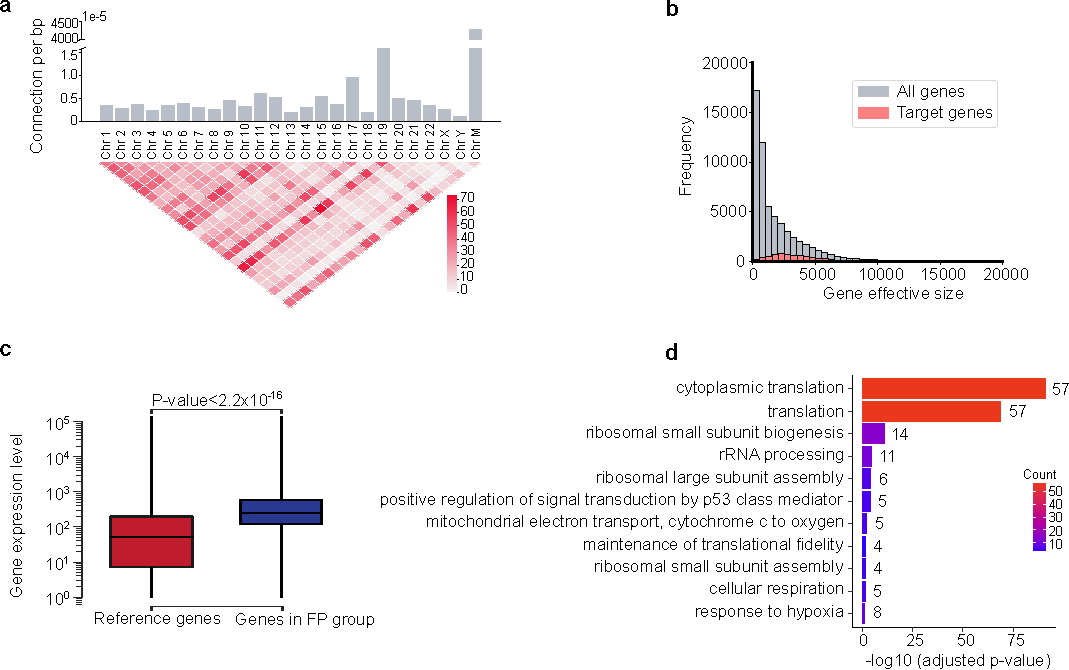
\includegraphics[height=0.65\columnwidth]{finals/sf2}
	\caption{ {\bf Analysis of \gls{drs} chimera artifacts and their genomic and transcriptomic characteristics in VCaP cells.} (a) Box plot comparing gene expression levels between all expressed genes (N=19,156) and genes affected by chimera artifacts (N=7,186) in the VCaP \gls{drs} dataset. Chimera artifacts-affected genes exhibit significantly higher expression levels (\(\textrm{p-value} < 2.2 \times 10^{-16}\)). (b) Distribution of gene effective sizes for all expressed genes and genes affected by chimera artifacts, indicating that the size distributions of genes impacted by chimera artifacts are comparable to those of all expressed genes. (c) Chromosomal distribution and interchromosomal connections from chimeric read artifacts arising from VCaP RNA004 \gls{drs}. The top bar plot shows the number of connections per kilobase for each chromosome, with higher bars indicating more frequent connections. The bottom heatmap visualizes the number of chimeric connections between chromosome pairs, with color intensity representing the connection frequency. (d) Number of detected transcripts across different isoform categories (\gls{fsm}, \gls{ism},  \gls{nic}, \gls{nnc}, and Other) from DeepChopper-identified chimeric read artifacts in VCaP RNA004 \gls{drs} data. DeepChopper-corrected reads resulted in a greater number of transcripts compared to adapter-trimmed reads by Dorado across all categories. }\label{fig:sf2}
\end{figure}


\begin{figure}[!h]
	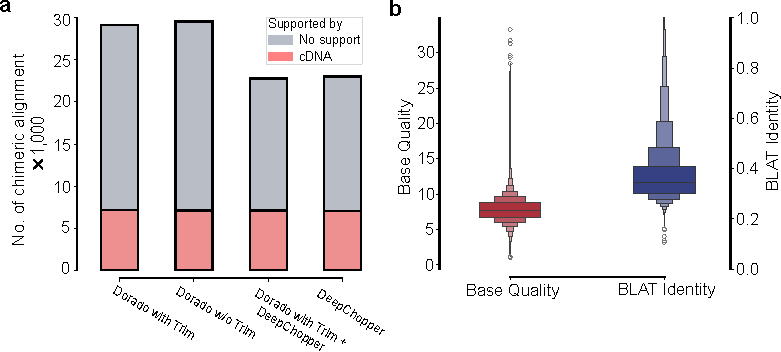
\includegraphics[height=1.45\columnwidth]{finals/sf3}
	\caption{ {\bf Analysis of gene fusions derived from chimeric read artifacts in \gls{drs}.} (a) Circos plot depicting chromosomal connections of gene fusions resulting from chimeric read artifacts in VCaP cells. Blue lines represent inter-chromosomal fusion events, while red lines indicate intra-chromosomal fusions. The outer track displays chromosomal ideograms labeled with respective chromosome numbers. (b) \gls{go} enrichment analysis of fusion genes derived from chimeric read artifacts identified by DeepChopper in \gls{drs} data from A549, HepG2, and HCT116 cell lines, and VCaP RNA004 \gls{drs} data. The table lists enriched \gls{go} terms of biological processes, associated genes, and the statistical significance (p-values) for each enrichment.}\label{fig:sf3}
\end{figure}


% \newpage

% \section{Supplementary information}

% \renewcommand{\figurename}{Supplementary Fig.}
% \renewcommand{\tablename}{Supplementary Table}


% If your article has accompanying supplementary file/s please state so here.
% Authors reporting data from electrophoretic gels and blots should supply the full unprocessed scans for key as part of their Supplementary information. This may be requested by the editorial team/s if it is missing.
% Please refer to Journal-level guidance for any specific requirements.


% \begin{table}
% 	\centering
% 	\caption{Hyperparameter ranges used}\label{tab:hyperparameter}
% 	\begin{tabular}{lc}
% 		\toprule
% 		                     & {$\sf DeepChopper$}               \\
% 		\midrule
% 		Parameters           & 1.6M                              \\
% 		Optimizer            & Adam                             \\
% 		Optimizer momentum   & $\beta_1$, $\beta_2$ = 0.9, 0.999 \\
% 		Training epoch       & 60                                \\
% 		Batch size           & 64                                \\
% 		Learning rate        & 2e-5                     \\
% 		LR scheduler         & ReduceLROnPlateau                 \\
% 		Weight decay (model) & 0                         \\
% 		Sequence lengths     & 32769                             \\
% 		\midrule
% 	\end{tabular}
% \end{table}

% \section*{Declarations}

% Some journals require declarations to be submitted in a standardised format. Please check the Instructions for Authors of the journal to which you are submitting to see if you need to complete this section. If yes, your manuscript must contain the following sections under the heading `Declarations':
%
%\begin{itemize}
%	\item Funding
%	\item Conflict of interest/Competing interests (check journal-specific guidelines for which heading to use)
%	\item Ethics approval and consent to participate
%	\item Consent for publication
%	\item Data availability
%	\item Materials availability
%	\item Code availability
%	\item Author contribution
%\end{itemize}

%
%\begin{appendices}
%	\printglossary[type=\acronymtype, title=Abbreviations]
%
%	\section{Section title of first appendix}\label{secA1}
%
%	An appendix contains supplementary information that is not an essential part of the text itself but which may be helpful in providing a more comprehensive understanding of the research problem or it is information that is too cumbersome to be included in the body of the paper.
%
%	%%=============================================%%
%	%% For submissions to Nature Portfolio Journals%%
%	%% please use the heading ``Extended Data''.   %%
%	%%=============================================%%
%
%	%%=============================================================%%
%	%% Sample for another appendix section			               %%
%	%%=============================================================%%
%
%	%% \section{Example of another appendix section}\label{secA2}%
%	%% Appendices may be used for helpful, supporting or essential material that would otherwise
%	%% clutter, break up or be distracting to the text. Appendices can consist of sections, figures,
%	%% tables and equations etc.


%\end{appendices}

%%===========================================================================================%%
%% If you are submitting to one of the Nature Portfolio journals, using the eJP submission   %%
%% system, please include the references within the manuscript file itself. You may do this  %%
%% by copying the reference list from your .bbl file, paste it into the main manuscript .tex %%
%% file, and delete the associated \verb+\bibliography+ commands.                            %%
%%===========================================================================================%%


%% if required, the content of .bbl file can be included here once bbl is generated
%%\input sn-article.bbl

\end{document}
